\documentclass[11pt, a4paper]{book}
\usepackage{physics}
\usepackage[margin=1in, headheight=14pt]{geometry}
\usepackage{amsfonts,amsmath,amssymb,suetterl}
\usepackage{lmodern}
\usepackage[T1]{fontenc}
\usepackage{mdwlist}
\usepackage[nodisplayskipstretch]{setspace}
\usepackage{float,graphicx}
\usepackage{epstopdf}
\usepackage{pgfplots}

%2
\usepackage{siunitx}
\usepackage{tkz-euclide}

\usetikzlibrary{calc}
\usetikzlibrary{positioning}
\usetikzlibrary{shapes.geometric}
%2 end

\pgfplotsset{compat = newest}
\usetikzlibrary{arrows.meta}

\setstretch{1.5}
\pagestyle{plain}

\newcommand{\lmrk}[2]{\hfill\textbf{Total for Question #1 is #2 marks}}
\newcommand{\mrk}[1]{\hfill\textbf{(#1)}}
\newcommand{\strch}{\vspace{\stretch{1}}}
\newcommand{\dline}{\tikz\draw[thick, dashed] (0,0) -- (3,0);}

\parindent 0ex
\setlength{\parskip}{1em}

\graphicspath{{images}}

\begin{document}
  \input{chapters/coverpage.tex}
  
\chapter{GCSE Revision - Algebraic Proof and Algebra in Context}

\begin{enumerate}
  \item Use algebra to prove that the sum of three consecutive whole numbers is always divisible by $3$.\strch
  \item Prove that $(2n + 3)^2 - (2n - 3)^2$ is a multiple of $8$ for all positive integer values of $n$.\strch
  \item The diagram shows a trapezium.
  \begin{figure}[H]
    \centering
    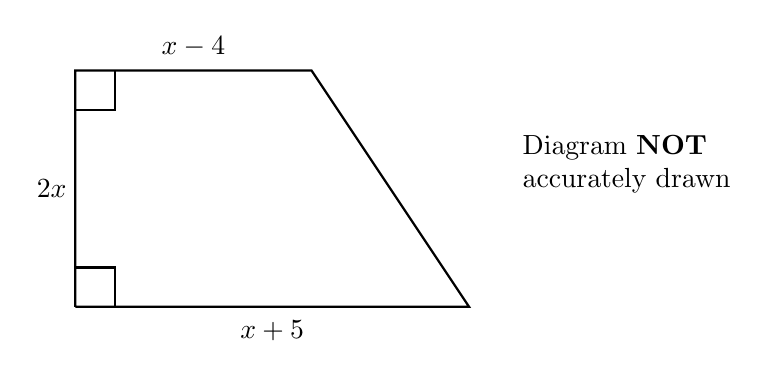
\begin{tikzpicture}
      \draw[thick] (0, 0) -- (5, 0) -- (3, 3) -- (0, 3) -- (0, 0);
      \node at (2.5, -0.3) {$x + 5$};
      \node at (-0.3, 1.5) {$2x$};
      \node at (1.5, 3.3) {$x - 4$};

      \draw[thick] (0, 0.5) -- (0.5, 0.5) -- (0.5, 0);
      \draw[thick] (0, 2.5) -- (0.5, 2.5) -- (0.5, 3);

      \node[label={[align=left]Diagram \textbf{NOT}\\accurately drawn}] at (7, 1.2) {};
    \end{tikzpicture}
  \end{figure}
  %
  All the measurements are in centimetres.\\
  The area of the trapezium is $351 cm^2$.
  \newpage
  \begin{enumerate}
    \item Show that $2x^2 + x - 351 = 0$.\mrk{2}\strch
    \item Work out the value of $x$.\mrk{3}\strch
  \end{enumerate}
  \item Here are two triangles $\vb{T_1}$ and $\vb{T_2}$.
  %
  \begin{figure}[H]
    \centering
    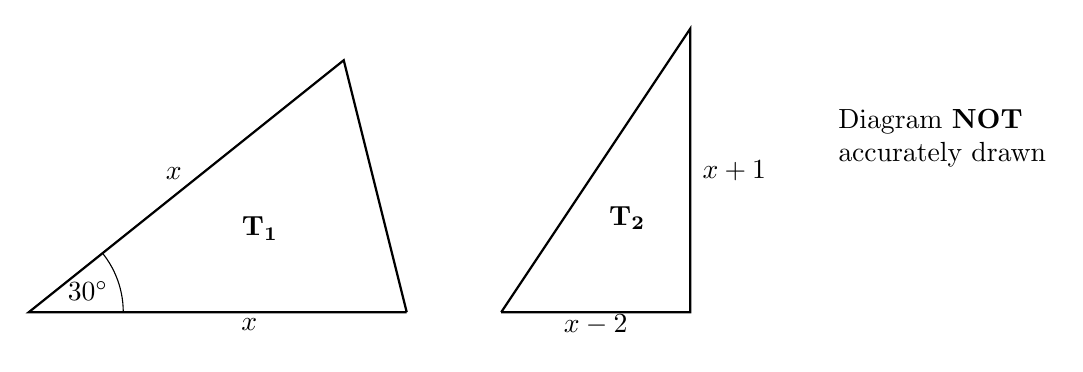
\begin{tikzpicture}[scale=0.8]
      \coordinate (A) at (-1, 0);
      \coordinate (B) at (-7, 0);
      \coordinate (C) at (-2, 4);

      \coordinate (X) at (0.5, 0);
      \coordinate (Y) at (3.5, 0);
      \coordinate (Z) at (3.5, 4.5);

      \coordinate (a1) at (-3.5, -0.2);
      \coordinate (a2) at (-4.7, 2.2);

      \coordinate (x1) at (2, -0.2);
      \coordinate (x2) at (4.2, 2.25);

      \coordinate (text) at (7.5, 2);

      \draw[thick] (A) -- (B) -- (C) -- (A);
      \draw[thick] (X) -- (Y) -- (Z) -- (X);

      \node at (-3.33, 1.33) {$\vb{T_1}$};
      \node at (2.5, 1.5) {$\vb{T_2}$};

      \begin{scope}
        \path[clip] (A) -- (B) -- (C);
        \draw (B) circle (15mm);
        \node at ($(B)+(20:10mm)$) {$\ang{30}$};
      \end{scope}

      \node at (a1) {$x$};
      \node at (a2) {$x$};

      \node at (x1) {$x - 2$};
      \node at (x2) {$x + 1$};

      \node[label={[align=left]Diagram \textbf{NOT} \\ accurately drawn}] at (text) {};
    \end{tikzpicture}
  \end{figure}
  %
  The lengths of the sides are in centimetres.\\
  The area of triangle $\vb{T_1}$ is equal to the area of triangle $\vb{T_2}$.\\
  Work out the value of $x$, giving your answer in the form $a + \sqrt{b}$ where $a$ and $b$ are integers.\strch
  \item Prove algebraically that the difference between the squares of any two consecutive integers is equal to the sum of these two integers.\strch
  \newpage
  \item \mbox{}
  \begin{figure}[H]
    \centering
    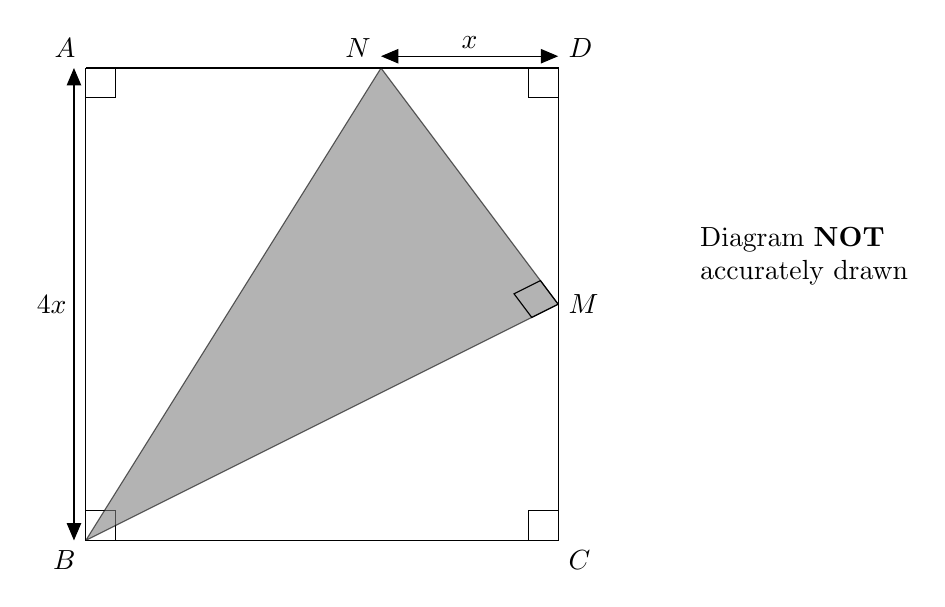
\begin{tikzpicture}[scale=1.5]
      \coordinate (B) at (0, 0);
      \coordinate (A) at (0, 4);
      \coordinate (C) at (4, 0);
      \coordinate (D) at (4, 4);

      \coordinate (M) at (4, 2);
      \coordinate (N) at (2.5, 4);

      \coordinate (varr1) at (0-0.1, 4);
      \coordinate (varr2) at (0-0.1, 0);

      \coordinate (harr1) at (4, 4+0.1);
      \coordinate (harr2) at (2.5, 4+0.1);

      \coordinate (t1) at (0, 2);
      \coordinate (t2) at (3.25, 4);

      \draw (A) -- (B) -- (C) -- (D) -- (A);

      \node at (A) [above left = 0.1mm of A] {$A$};
      \node at (B) [below left = 0.1mm of B] {$B$};
      \node at (C) [below right = 0.11mm of C] {$C$};
      \node at (D) [above right = 0.1mm of D] {$D$};

      \tkzMarkRightAngle (A,B,C);
      \tkzMarkRightAngle (B,C,D);
      \tkzMarkRightAngle (D,A,B);
      \tkzMarkRightAngle (A,D,C);

      \draw[color=black, fill=gray, opacity=0.6] (B) -- (M) -- (N) -- (B);
      \tkzMarkRightAngle (B,M,N);

      \node at (M) [right = 0.1mm of M] {$M$};
      \node at (N) [above left = 0.1mm of N] {$N$};

      \draw[>=triangle 45, <->] (varr1) -- (varr2);
      \draw[>=triangle 45, <->] (harr1) -- (harr2);

      \node at (t1) [left = 1.2mm of t1] {$4x$};
      \node at (t2) [above = 1.2mm of t2] {$x$};

      \node[label={[align=left]Diagram \textbf{NOT} \\ accurately drawn}] at (M) [right = 3cm of M] {};
    \end{tikzpicture}
  \end{figure}
  %
  $ABCD$ is a square with a side length of $4x$.\\
  $M$ is the midpoint of $DC$.\\
  $N$ is the point on $AD$ where $ND = x$.\par
  $BMN$ is a right-angled triangle.\par
  Find an expression, in terms of $x$, for the area of triangle $BMN$.\\
  Give your expression in its simplest form.\strch
  \newpage
  \item \mbox{}
  \begin{figure}[H]
    \centering
    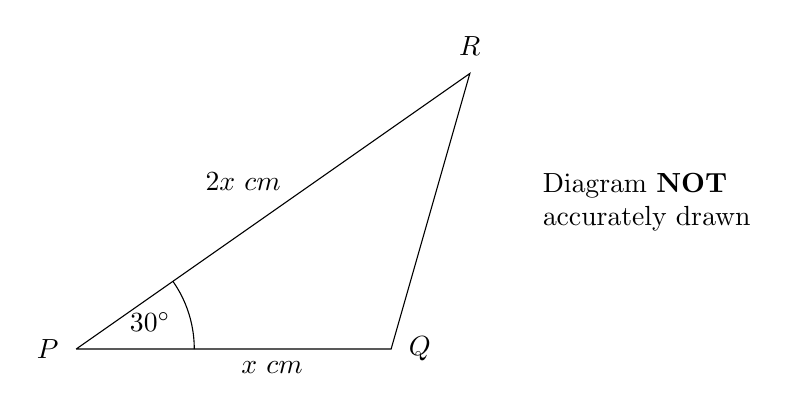
\begin{tikzpicture}
      \coordinate (P) at (0, 0);
      \coordinate (Q) at (4, 0);
      \coordinate (R) at (5, 3.5);

      \draw (P) -- (Q) -- (R) -- (P);

      \node at (P) [left = 1mm of P] {$P$};
      \node at (R) [above = 1mm of R] {$R$};
      \node at (Q) [right = 1mm of Q] {$Q$};

      \begin{scope}
        \path[clip] (R) -- (P) -- (Q);
        \draw (P) circle (15mm);
        \node at ($(P)+(20:10mm)$) {$\ang{30}$};
      \end{scope}

      \node at ($(P)+(45:3cm)$) {$2x\ cm$};
      \node at ($(P)+(-5.5:2.5cm)$) {$x\ cm$};

      \node[label={[align=left]Diagram \textbf{NOT} \\ accurately drawn}] at (R) [below right = 3cm of R] {};
    \end{tikzpicture}
  \end{figure}
  %
  $PQ = x\ cm$\\
  $PR = 2x\ cm$\\
  Angle $QPR = \ang{30}$\par
  The area of triangle $PQR = A\ cm^2$\\
  Show that $x = \sqrt{2A}$.\strch
  \item \mbox{}
  \begin{figure}[H]
    \centering
    \begin{tikzpicture}[scale=1.2]
      \coordinate (P) at (0, 0);
      \coordinate (Q) at (6, 0);
      \coordinate (R) at (0, 3);

      \draw (P) -- (Q) -- (R) -- (P);

      \tkzMarkRightAngle (R,P,Q);

      \node at ($(P)+(32:3.7cm)$) {$3x + 1$};
      \node at ($(P)+(-5.5:2.5cm)$) {$3x$};
      \node at ($(P)+(110:1.5cm)$) {$x-1$};

      \node[label={[align=left]Diagram \textbf{NOT} \\ accurately drawn}] at (Q) [above right = 3cm of Q] {};
    \end{tikzpicture}
  \end{figure}
  %
  In the diagram, all the measurements are in metres.\par
  The perimeter of the triangle is $56$ m.\\
  The area of the triangle is $A$ $\text{m}^2$.\par
  Work out the value of $A$.\strch
  \newpage
  \item \mbox{}
  \begin{figure}[H]
    \centering
    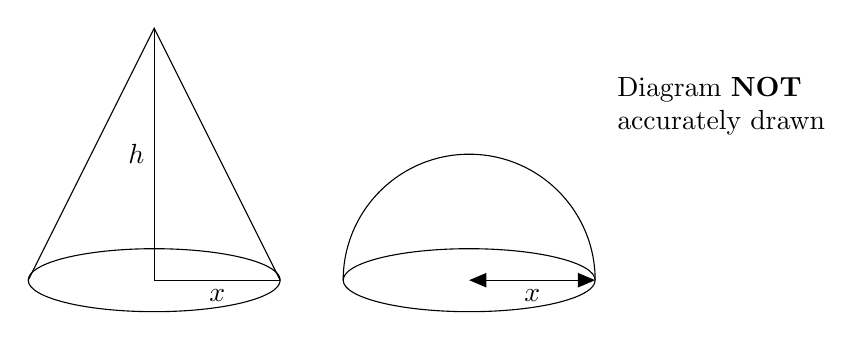
\begin{tikzpicture}[scale=0.8]
      \draw (0,0) circle (2cm and 0.5cm);
      \draw(2,0) -- (0,4) -- (-2,0);
      \draw (2,0) -- node[below] {$x$} (0,0) -- node[left] {$h$} (0,4) ;

      \draw (5,0) circle (2cm and 0.5cm);
      \draw (3,0) arc (180:0:2);

      \draw[>=triangle 45, <->] (5,0) -- node[below] {$x$} (7,0);

      \node[label={[align=left]Diagram \textbf{NOT} \\ accurately drawn}] at (9, 2) {};
    \end{tikzpicture}
  \end{figure}
  %
  The diagram shows a solid cone and a solid hemisphere.\\
  The cone has a base of radius $x$ cm and a height of $h$ cm.\\
  The hemisphere has a base of radius $x$ cm.\\
  The surface area of the cone is equal to the surface area of the hemisphere.\par
  Find an expression for $h$ in terms of $x$.\strch
  \item Umar thinks $(a + 1)^2 = a^2 + 1$ for all values of $a$.
  \begin{enumerate}
    \item Show that Umar is wrong.\mrk{2}\strch
    \item Here are two right-angled triangles.\\
    All the measurements are in centimetres
    \begin{figure}[H]
      \centering
      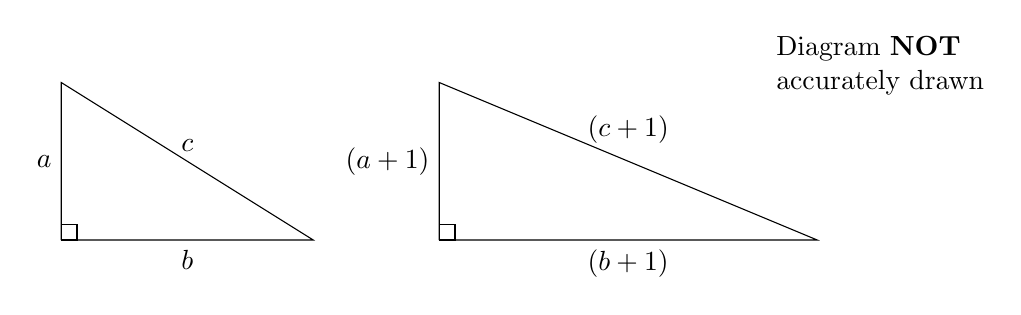
\begin{tikzpicture}[scale=0.8]
        \coordinate (A1) at (0, 0);
        \coordinate (B1) at (4, 0);
        \coordinate (C1) at (0, 2.5);

        \coordinate (A2) at (6, 0);
        \coordinate (B2) at (12, 0);
        \coordinate (C2) at (6, 2.5);

        \draw (A1) -- node[left] {$a$} (C1) -- node[above] {$c$} (B1) -- node[below] {$b$} (A1);
        \tkzMarkRightAngle (B1,A1,C1);

        \draw (A2) -- node[left] {$(a+1)$} (C2) -- node[above=1mm] {$(c+1)$} (B2) -- node[below] {$(b+1)$} (A2);
        \tkzMarkRightAngle (B2,A2,C2);

        \node[label={[align=left]Diagram \textbf{NOT} \\ accurately drawn}] at (13, 2) {};
      \end{tikzpicture}
    \end{figure}
    %
    Show that $2a + 2b + 1 = 2c$. $a,\ b$ and $c$ cannot all be integers.\mrk{3}\strch
    \newpage
    \item Explain why.\mrk{1}\strch
  \end{enumerate}
  \item The diagram below shows a large rectangle of length $(2x + 6)$ cm and width $x$ cm. A smaller rectangle of length $x$ cm and width $3$ cm is cut out and removed.
  %
  \begin{figure}[H]
    \centering
    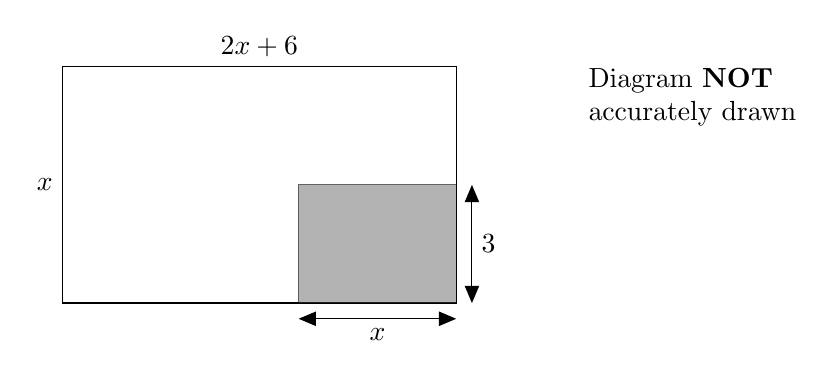
\begin{tikzpicture}
      \coordinate (A1) at (0, 0);
      \coordinate (B1) at (5, 0);
      \coordinate (C1) at (5, 3);
      \coordinate (D1) at (0, 3);

      \coordinate (A2) at (3, 0);
      \coordinate (B2) at (3, 1.5);
      \coordinate (C2) at (5, 1.5);

      \coordinate (varr1) at (3, -0.2);
      \coordinate (varr2) at (5, -0.2);

      \coordinate (harr1) at (5.2, 0);
      \coordinate (harr2) at (5.2, 1.5);

      \draw (A1) -- (B1) -- (C1) -- node[above] {$2x + 6$} (D1) -- node[left] {$x$} (A1);
      \draw[color=black, fill=gray, opacity=0.6] (A2) -- (B2) -- (C2) -- (B1) -- (A2);

      \draw[>=triangle 45, <->] (varr1) -- node[below] {$x$} (varr2);
      \draw[>=triangle 45, <->] (harr1) -- node[right] {$3$} (harr2);
    
      \node[label={[align=left]Diagram \textbf{NOT} \\ accurately drawn}] at (8, 2) {};
    \end{tikzpicture}
  \end{figure}
  %
  The area of the shape that is left is $100$ $\text{cm}^2$
  \begin{enumerate}
    \item Show that $2x^2 + 3x - 100 = 0$.\mrk{3}\strch
    \item Calculate the length of the smaller rectangle. Give your answer correct to $3$ significant figures.\mrk{4}\strch
  \end{enumerate}
  \newpage
  \item \mbox{}
  \begin{figure}[H]
    \centering
    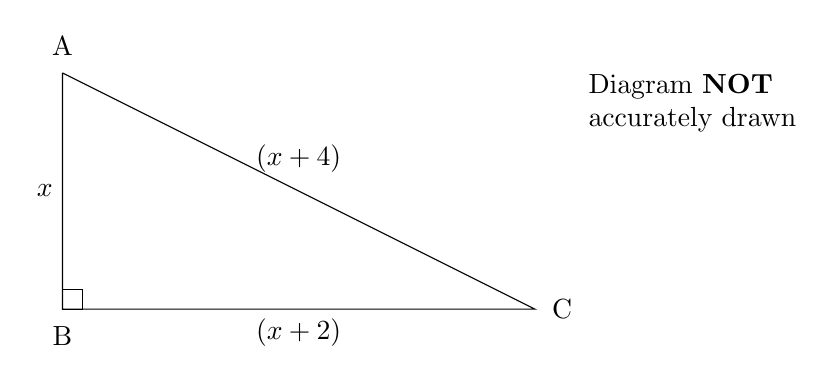
\begin{tikzpicture}
      \coordinate (B1) at (0, 0);
      \coordinate (A1) at (0, 3);
      \coordinate (C1) at (6, 0);

      \draw (A1) -- node[left] {$x$} (B1) -- node[below] {$(x+2)$} (C1) -- node[above=1.1mm] {$(x+4)$} (A1);
      \tkzMarkRightAngle (A1,B1,C1);

      \node[label=above:A, scale=0.75] (A1) at (A1) {};
      \node[label=below:B, scale=0.75] (B1) at (B1) {};
      \node[label=right:C, scale=0.75] (C1) at (C1) {};

      \node[label={[align=left]Diagram \textbf{NOT} \\ accurately drawn}] at (8, 2) {};
    \end{tikzpicture}
  \end{figure}
  %
  ABC is a right-angled triangle.\\
  All the measurements are in centimetres.\par
  $AB = x$\\
  $BC = (x + 2)$\\
  $AC = (x + 4)$
  \begin{enumerate}
    \item Show that $x^2 - 4x - 12 = 0$.\mrk{3}\strch
    \item \hfill\mrk{4}
    \begin{enumerate}
      \item Solve $x^2 - 4x - 12 = 0$\strch
      \item Hence, write down the length of $AC$.\strch
    \end{enumerate}
  \end{enumerate}
  \item Prove that the difference between the squares of two consecutive odd numbers is a multiple of $8$.\strch
  \newpage
  \item Prove that $n^2 + n + 1$ is always odd for all integers $n$.\strch
  \item Factorise $2t^2 + 5t + 2$. Hence explain why $2t^2 + 5t + 2$ can never be a prime number for any positive whole number value of $t$.\strch
\end{enumerate}
  
\chapter{GCSE Revision - Algebra - (Excluding Geometric problems and proofs)}
\begin{enumerate}
  \item
  \begin{enumerate}
    \item Simplify $x^7 \times x^3$\strch
    \item Simplify $(m^4)^3$\strch
    \item Simplify $\dfrac{36af^8}{12a^5f^2}$\strch\\ \vspace*{0pt}\lmrk{1}{7}
  \end{enumerate}
  \pagebreak
  \item %
  \begin{enumerate}
    \item Solve $\dfrac{4(8x - 2)}{3x} = 10$\mrk{3}\strch
    \item Write as a single fraction in its simplest form\mrk{3}
    $$
    \frac{2}{y + 3} - \frac{1}{y - 6}
    $$
    \strch
  \end{enumerate}
  %
  \item Solve the simultaneous equations
  \begin{align*}
    3x + 4y = 5\\
    2x - 3y = 9
  \end{align*}
  \hfill$x =\ $\dline\\
  \vspace*{0pt}\hfill$y =\ $\dline\\
  \vspace*{0pt}\lmrk{3}{4}
  \strch
  \item %
  \begin{align*}
    &A = 4bc\\
    &A = 100\\
    &b = 2
  \end{align*}
  \begin{enumerate}
    \item Work out the value of $c$.\mrk{2}\strch\newpage
    \item Make $k$ the subject of the formula, $m = \sqrt{\dfrac{k+1}{4}}$.\mrk{3}\strch
  \end{enumerate}
  \item Solve $\dfrac{4x - 1}{5} + \dfrac{x + 4}{2} = 3$\mrk{3}\strch\\
  \vspace*{0cm}\hfill$x =\ $\dline
  \item %
  \begin{enumerate}
    \item Simplify $a^4\times a^5$\mrk{1}\strch
    \item Simplify $\dfrac{45e^6f^8}{5ef^2}$\mrk{2}\strch
    \item Write down the value of $9^{\frac{1}{2}}$.\mrk{1}\strch
  \end{enumerate}
  \newpage
  \item Solve the simultaneous equations\mrk{6}
  \begin{align*}
    x^2 + y^2 &= 9\\
    x + y &= 2
  \end{align*}
  Give your answers correct to 2 decimal places.\strch\\
  \vspace*{0pt}\hfill$x =\ $\dline\hspace{0.2cm} $y =\ $\dline\\
  \vspace*{0pt}\hfill or $x =\ $\dline\hspace{0.2cm} $y =\ $\dline
  \item Make $p$ the subject of the formula $y = 3p^2 - 4$.\mrk{3}\strch
  \item %
  \begin{enumerate}
    \item Factorise	$6 + 9x$.\mrk{1}\strch
    \item Factorise	$y^2 - 16$.\mrk{1}\strch
    \item Factorise	$2p^2 - p - 10$.\mrk{2}\strch
  \end{enumerate}
  \newpage
  \item Solve $\dfrac{2 - y}{5} = 1$.\mrk{5}\strch\\\vspace*{0pt}\hfill $y =\ $\dline
  \item The expression $x^2 - 8x + 21$ can be written in the form $(x - a)^2 + b$ for all values of $x$.
  \begin{enumerate}
    \item Find the value of $a$ and the value of $b$.\mrk{3}\strch\\
    \vspace*{0pt}\hfill $a =\ $\dline\\
    \vspace*{0pt}\hfill $b =\ $\dline
    \suspend{enumerate}
    The equation of a curve is $y = f(x)$ where $f(x) = x^2 - 8x + 21$. The diagram shows part of a sketch of the graph of $y = f(x)$.
    \begin{figure}[H]
      \centering
      \begin{tikzpicture}
        \begin{axis}[
            xmin = -1, xmax = 10,
            ymin = -2, ymax = 30,
            xticklabels = {},
            yticklabels = {},
            axis lines = middle,
            xlabel = {$x$},
            ylabel = {$y$},
          ]
          % Plot a function
          \addplot[
            domain = -0.8:8.8,
            samples = 200,
            smooth,
            thick,
          ] {x^2 - 8*x + 21};
          \node at (7.5, 28) {$y = f(x)$};
          \node at (-0.4, -1) {$O$};
          \node at (4, 3) {$M$};
          \addplot[
            mark=x,
            mark size=6pt
          ]
          coordinates {
            (4, 5)
          };
        \end{axis}
      \end{tikzpicture}
    \end{figure}
    The minimum point of the curve is $M$.
    \resume{enumerate}
    \item Write down the coordinates of $M$.\mrk{1}\strch\\
    \vspace*{0pt}\hfill (
      \tikz\draw[thick, dashed] (0,0) -- (1.5,0);, \tikz\draw[thick, dashed] (0,0) -- (1.5,0);
    )
  \end{enumerate}
  \newpage
  \item Simplify $\dfrac{4(x + 5)}{x^2 + 2x - 15}$.\mrk{2}\strch
  \item Solve the simultaneous equations\mrk{4}
  \begin{align*}
    4x + 7y &= 1\\
    3x + 10y &= 15
  \end{align*}\strch\\
  \vspace*{0pt}\hfill$x =\ $\dline\\
  \vspace*{0pt}\hfill$y =\ $\dline
  \begin{enumerate}
    \item Solve 	$2x^2 + 9x - 7 = 0$. Give your solutions correct to 3 significant figures.\mrk{3}\strch
    \item Solve $\dfrac{2}{y^2} + \dfrac{9}{y} - 7 =0$. Give your solutions correct to 3 significant figures.\mrk{2}\strch
  \end{enumerate}
  \item Simplify $\dfrac{x + 1}{2} + \dfrac{x + 3}{3}$.\mrk{3}\strch
  \newpage
  \item %
  \begin{enumerate}
    \item %
    \begin{enumerate}
      \item Factorise $2t^2 + 5t + 2$.\strch
      \item $t$ is a positive whole number.\par
      The expression $2t^2 + 5t + 2$ can never have a value that is a prime number. Explain why.\mrk{3}\strch
    \end{enumerate}
  \end{enumerate}
  \item Make $t$ the subject of the formula\mrk{4} $$p = \frac{3-2t}{4 + t}$$\strch
  \item Solve $\dfrac{5(2x + 1)^2}{4x + 5} = 5x - 1$.\mrk{5}\strch
  \item Solve the equations\mrk{4}
  \begin{align*}
    3x + 5y &= 19\\
    4x - 2y &= -18
  \end{align*}
  \strch\\
  \vspace*{0pt}\hfill$x =\ $\dline\\
  \vspace*{0pt}\hfill$y =\ $\dline
  \item Solve the equation 	$5x^2 + 8x - 6 = 0$. Give each solution correct to 2 decimal places.\mrk{3}\strch
  \newpage
  \item %
  \begin{enumerate}
    \item On the number line below, show the inequality $-2 < y < 3$.\mrk{1}
    \begin{figure}[H]
      \centering
      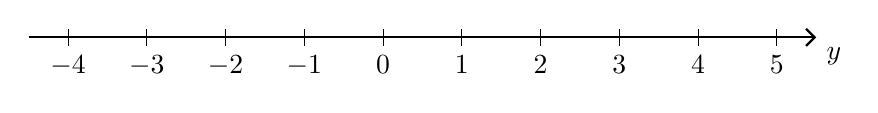
\begin{tikzpicture}
        \draw[-Straight Barb, thick] (-4.5, 0) -- (5.5, 0) node[anchor=north west] {$y$};
        \foreach \x in {-4, -3, -2, -1, 0, 1, 2, 3, 4, 5}
          \draw (\x cm, 3pt) -- (\x cm, -3pt) node[anchor=north] {$\x$};
      \end{tikzpicture}
    \end{figure}\strch
    \item Here is an inequality, in $x$, shown on a number line.\mrk{2}
    \begin{figure}[H]
      \centering
      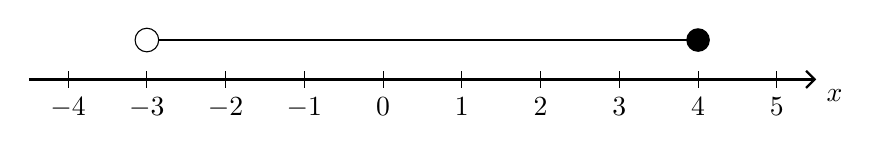
\begin{tikzpicture}
        \draw[-Straight Barb, thick] (-4.5, 0) -- (5.5, 0) node[anchor=north west] {$x$};
        \foreach \x in {-4, -3, -2, -1, 0, 1, 2, 3, 4, 5}
          \draw (\x cm, 3pt) -- (\x cm, -3pt) node[anchor=north] {$\x$};
        \draw[thick] (-3, 0.5) -- (4, 0.5);
        \filldraw[fill=white, draw=black] (-3, 0.5) circle (0.15cm);
        \fill[black] (4, 0.5) circle (0.15cm);
      \end{tikzpicture}
    \end{figure}
    Write down the inequality.\strch
    \item Solve the inequality $4t - 5 > 9$.\mrk{2}\strch
  \end{enumerate}
  \item %
  \begin{enumerate}
    \item Factorise fully $2x^2 - 4xy$.\mrk{2}\strch
    \item Factorise $p^2 - 6p + 8$.\mrk{2}\strch
    \item Simplify $\dfrac{(x+2)^2}{x+2}$.\mrk{1}\strch
    \item Simplify $2a^2b \times 3a^3b$.\mrk{2}\strch
  \end{enumerate}
  \newpage
  \item Solve $3x^2 - 4x - 2 = 0$ Give your solutions correct to 3 significant figures.\mrk{3}\strch
  \item Make $t$ the subject of the formula $2(d - t) = 4t + 7$.\mrk{3}\strch\\
  \vspace*{0pt}\hfill$t =\ $\dline
  \item %
  \begin{enumerate}
    \item Simplify fully $\dfrac{x^2 + 3x - 4}{2x^2 - 5x + 3}$.\mrk{3}\strch
    \item Write $\dfrac{4}{x + 2} + \dfrac{3}{x - 2}$ as a single fraction in its simplest form.\mrk{3}\strch
  \end{enumerate}
  \item %
  \begin{enumerate}
    \item Factorise $x^2 + px + qx + pq$.\mrk{2}\strch
    \item Factorise $m^2 - 4$.\mrk{1}\strch
    \item Write as a single fraction in its simplest form $\dfrac{2}{x - 4} - \dfrac{1}{x + 3}$.\mrk{3}\strch
  \end{enumerate}
  \newpage
  \item Find the exact solutions of $x + \dfrac{3}{x} = 7$.\mrk{3}\strch
  \item 	$-2 \leq n < 5$, $n$ is an integer.
  \begin{enumerate}
    \item Write down all the possible values of $n$.\mrk{2}\strch
    \item Solve the inequality	$4x + 1 > 11$.\mrk{2}\strch
  \end{enumerate}
  \item Simplify $(2n^3)^4$.\mrk{2}\strch
  \item %
  \begin{enumerate}
    \item Factorise $2x^2 - 9x + 4$.\mrk{2}\strch\\
    Hence, or otherwise,
    \item Solve $2x^2 - 9x + 4 = (2x - 1)^2$\mrk{4}\strch
  \end{enumerate}
  \newpage
  \item $y = p - 2qx^2$\par
  $p = -10,\quad q = 3,\quad	x = -5$    
  \begin{enumerate}
    \item Work out the value of $y$.\mrk{2}\strch
    \item Rearrange $y = p - 2qx^2$ to make $x$ the subject of the formula.\mrk{3}\strch
  \end{enumerate}
  \item The diagram shows the graph of $y = x^2 - 5x - 3$
  \begin{figure}[H]
    \centering
    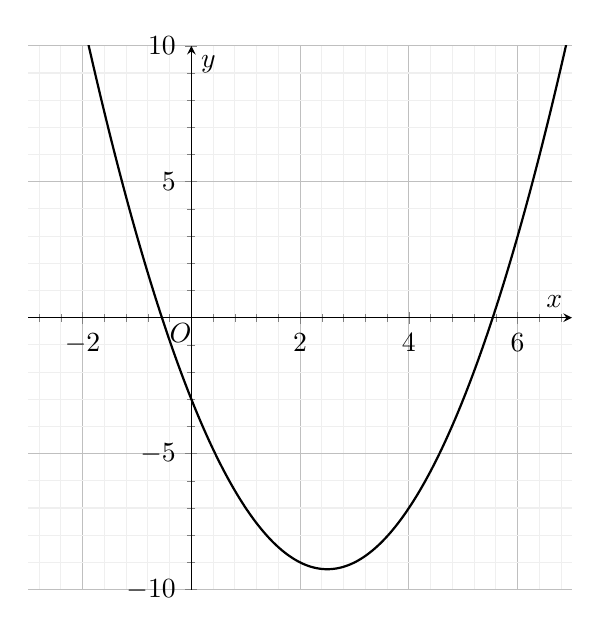
\begin{tikzpicture}
      \begin{axis}[
          xmin = -3, xmax = 7,
          ymin = -10, ymax = 10,
          grid = both,
          minor tick num = 4,
          major grid style = {lightgray},
          minor grid style = {lightgray!25},
          axis lines = center,
          width = 0.7\textwidth,
          height = 0.7\textwidth,
          xlabel = {$x$},
          ylabel = {$y$},
        ]
        % Plot a function
        \addplot[
          domain = -2:7,
          samples = 500,
          smooth,
          thick,
        ] {x^2 - 5*x - 3};
        \node at (-0.2, -0.55) {$O$};
      \end{axis}
    \end{tikzpicture}
  \end{figure}
  \newpage
  \begin{enumerate}
    \item Use the graph to find estimates for the solutions of.\mrk{3}
    \begin{enumerate}
      \item $x^2 - 5x - 3 = 0$.\strch
      \item $x^2 - 5x - 3 = 6$.\strch
    \end{enumerate}
    \item Use the graph to find estimates for the solutions of the simultaneous equations\mrk{3}
    \begin{align*}
      y &= x2 - 5x - 3\\
      y &= x - 4
    \end{align*}\strch
  \end{enumerate}
  \item The table shows six expressions. $n$ is a positive integer.\par
  \begin{table}[H]
    \centering
    \resizebox{0.85\textwidth}{!}{%
    \begin{tabular}{|c|c|c|c|c|c|} 
      \hline
      $2n - 3$ & $3n - 2$ & $3(n + 4)$ & $4n + 1$ & $4(3n + 1)$ & $2n + 1$ \\ 
      \hline
    \end{tabular}}
  \end{table}
  \begin{enumerate}
    \item From the table, write the expression whose value is\mrk{2}
    \begin{enumerate}
      \item always even.
      \item always a multiple of 3.
    \end{enumerate}
    \item From the table, write the expression which is a factor of $4n^2 - 1$.\mrk{1}\strch
  \end{enumerate}
  \item Solve the equation $\dfrac{x}{2} - \dfrac{2}{x + 1} = 1$.\mrk{4}\strch
  \newpage
  \item Make $k$ the subject of the formula $t = \dfrac{k}{k - 2}$.\mrk{4}\strch
  \item %
  \begin{enumerate}
    \item Simplify completely $\dfrac{12xy^3}{3x^2y^3}$.\mrk{2}\strch
  \end{enumerate}
  \item %
  \begin{enumerate}
    \item Expand and simplify $(2x + 4y)(4x - 5y)$.\mrk{2}\strch
    \item Simplify fully $\dfrac{(x + 10)^5}{(x + 10)^4}$.\mrk{1}\strch
    \item Simplify fully $\dfrac{x^2 - 25}{x^2 + 7x + 10}$\mrk{3}\strch
    \item For all values of $x,\ x^2 + 6x - 2 = (x + p)^2 + q$. Find the value of $p$ and the value of $q$.\mrk{3}\strch\\
    \vspace*{0pt}\hfill $p=\ $
      \tikz\draw[thick, dashed] (0,0) -- (1.5,0);, $q=\ $ \tikz\draw[thick, dashed] (0,0) -- (1.5,0);
  \end{enumerate}
  \newpage
  \item Make $v$ the subject of the formula $t = \dfrac{v}{5} + 2$.\mrk{2}\\[2cm]
  \vspace*{0pt}\hfill $v=\ $\dline
\end{enumerate}
\end{document}